\section{L'arithmétique de Peano}
\subsection{Introduction à l'arithmétique}

À l'époque de la Grèce Antique, les nombres en mathématique ne se limitaient qu'aux entiers naturels. \newline
En effet, même les nombres décimaux étaient représentés sous forme d'entier en changeant  la base. \newline
Par exemple : si une longueur géométrique mesurait $1,9 m$ alors à la place on disait que la longueur mesurait $19 dm$ et on adaptait ainsi toutes les autres mesures. \newline
\newline
(Anecdote : c'est par cette logique qu'un Pythagoricien a démontré l'existence de nombres irrationnels, des nombres ne pouvant pas être ramenés à une base car possédant une infinité de chiffres derrière la virgule \ !) \newline

Par conséquent, les opérations élementaires de l'arithmétique étaient l'addition, la soustraction, la multiplication et la division. \newline
Alors que l'addition et la multiplication sont des opérations triviales conservant la qualité d'entier d'un nombre, pour la division c'est une autre paire de manche (concernant la soustraction, l'introduction des entiers relatifs réglera ce problème). \newline
La division classique était appelée à l'époque "Division Euclidienne". \newline
Créée par le mathématicien Grec \textit{Euclide}\ref{itm:Euclide}, cette division, bien que réadaptée au fil du temps pour s'appliquer aux entiers relatifs,  permettait de ne pas avoir de partie fractionelle car il définissait une division comme étant un quotient et un reste.

\begin{theorem}
\textbf{Division Euclidienne} (Version adaptée) : \newline
Soient $a \in \ens{Z}$ et $b \in \ens{N}$, alors $\exists! (q,r) \in \ens{Z} \times \ens{N}$ avec $0 \leq r < b$ tels que : \newline
$$a = bq + r$$
\end{theorem}

(Note : la démonstration étant assez longue et hors-sujet, nous vous laissons voir la référence \ref{itm:DivEuc}) \newline

Cette définition de la division euclidienne peut sembler quelque peu abrupte, mais en fait cela est équivalent à la division euclidienne que l'on faisait en primaire ! (voir figure \ref{fig:DivEuc}) \newline

a := Dividende / b := Diviseur / q := Quotient / r := Reste
\begin{figure}[h]
    \centering
    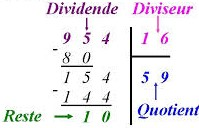
\includegraphics{division_euclidienne.jpg}
    \caption{Division euclidienne}
    \label{fig:DivEuc}
\end{figure}
\newline \newline \newline
Au cours du temps l'arithmétique n'a fait que se complexifier et se mélanger avec d'autres disciplines et créer d'autres types d'arithmétiques :

\begin{itemize}
    \item l'arithmétique modulaire \ref{itm:AriMod}
    \item la théorie algébrique des nombres \ref{itm:AriAlg}
    \item l'arithmétique des polynômes \ref{itm:AriPol}
\end{itemize}

Mais, pendant la crise des fondements\ref{itm:CriFon}, le mathématicien italien \textit{Giuseppe Peano}\ref{itm:Peano} décida en 1889 de formaliser l'arithmétique en créant un système axiomatique que l'on appela "l'arithmétique de Peano". \newline
C'est le début des fondations de l'arithmétique moderne, mais, avant de s'atteler à cette arithmétique, nous devons d'abord introduire les symboles de la logique mathématique.

\subsection{Introduction aux symboles}

Un théorème de l'arithmétique de Peano est forcément écrit par ces symboles :

\paragraph{Opérateurs et inconnues}
\textbf{:} \newline
Les 2 opérateurs : $+ \ \times$ \newline
Des lettres, que ce soit, latines, grecques, parfois avec des indexations, majuscules ou minuscules : $x$, $y$, $\delta$, $x_n$ \ldots

\paragraph{Quantificateurs :}
Les 2 uniques quantificateurs et leur variation : \newline
$\forall$ : Pour tout / Quel que soit \newline
$\exists$ : Il existe \newline
$\exists!$ : Il existe un unique 

\paragraph{symboles logiques :}
Les symboles de la logique classique : \newline
$\implies$ : implication \newline
$\Longleftrightarrow$ : équivalence \newline
$\wedge$ : et \newline
$\vee$ : ou \newline
$\neg$ : négation \newline
$=$ : égalité \newline
$P(x, \ldots ,x_n)$ : Une propriété dépendant de $n$ variables \newline

\paragraph{symboles de Peano :}
Alors que les opérateurs, les quantificateurs et les symboles logiques peuvent être trouvés dans d'autres théories, les 2 prochains symboles sont propres à l'arithmétique de Peano : \newline \newline
1) la constante $0$ : seul chiffre pouvant être écrit car son existence est assumée par l'ensemble axiomatique de Peano (nous traiterons plus profondément de ce sujet dans la section \ref{sec:AxioPea}). \newline \newline
2)La fonction $S$ (Successeur). \newline
On pourrait intuitivement la définir comme :
\begin{align*}
    S : \ & \ens{N} \ \to \ \ens{N} \\
        & n \ \mapsto \ n+1 \\
\end{align*}
(Note : il faut bien comprendre qu'ici la fonction est une idée, il ne faut pas l'imaginer dans le sens d'une fonction à proprement parler. Nous l'avons mise sous cette forme pour aider à l'intuition mais à ce stade de la théorie, une fonction n'est même pas définie, c'est donc un non-sens de définir un axiome sur quelque chose qui n'existe pas.)


\subsection{Les axiomes de l'arithmétique de Peano}
\subsubsection{Définition d'un axiome et d'un système axiomatique}

Avant de se lancer à bras le corps dans le système axiomatique de Peano, il est important d'avoir une compréhension complète de ce que sont un axiome et un système axiomatique. \newline

\begin{definition} \label{def:Axiome}
\textbf{Axiome} \ref{itm:Axiome} : \newline
Proposition considérée comme évidente, admise sans démonstration.
\end{definition}
\begin{definition} \label{def:SysAxi}
\textbf{Système axiomatique} \ref{itm:SysAxi} : \newline
Ensemble d'axiomes dont certains ou tous les axiomes peuvent être utilisés logiquement pour dériver des théorèmes.
\end{definition}

Analysons plus en détail leur signification : \newline
Premièrement, avant de comprendre la définition, il est important de comprendre la motivation d'une telle définition. \newline
Si l'on devait faire une analogie, l'ensemble des théories mathématiques équivaudrait à un arbre. Chaque branche est un théorème et chaque feuille ou branche liée à cette dernière est un corrolaire ou un nouveau théorème. \newline
En effet, chaque théorème utilise des informations issues d'un autre théorème prouvé préalablement (et parfois même pas prouvé d'ailleurs...!) et ainsi de suite. \newline
Par conséquent, les axiomes sont les racines de cet arbre, les "théorèmes originaux". \newline
C'est pourquoi, d'après la définition \ref{def:Axiome}, les axiomes sont des propositions, car s'il existait une démonstration, ils seraient des théorèmes et non des axiomes. \newline
\newline
Ainsi, avec plusieurs axiomes on forme un système axiomatique, et c'est en combinant ces axiomes de manière logique qu'on peut ainsi créer des théorèmes, et ainsi de suite. \newline
Un système axiomatique est la base d'une théorie (exemple : la théorie des ensembles ZFC (\ref{itm:ThrZFC}) ou l'arithmétique de Peano). Ils diffèrent selon les théories, qui sont parfois plus ou moins complètes (on les appelle des théories de premier ordre (\ref{itm:CalPre}) par exemple). \newline
Le plus important pour une théorie est que'elle soit cohérente (même si on ne peut pas prouver qu'elle l'est ou non (\ref{itm:ThmGdl}) !).

\begin{definition}
\textbf{cohérence} : \newline
La cohérence est la propriété d'une théorie exempte de contradiction.
\end{definition}

Plus intuitivement, un système axiomatique est dit incohérent s'il est possible de former 2 théorèmes qui prouvent quelque chose et son contraire. \newline
Pour bien comprendre le principe d'un système axiomatique, regardons un petit exemple :

\begin{example}
Créons une théorie : \newline
Axiome 1 : les mammifères ne pondent pas des œufs. \newline
Axiome 2 : les ornithorynques sont des mammifères. \newline
Axiome 3 : les ornithorynques pondent des œufs. \newline

Nous venons de créer un système axiomatique avec ces 3 axiomes, regardons les théorèmes que l'on peut faire avec : \newline
\newline
Théorème : les ornythorinques ne sont pas des mammifères (axiome 1+3). \newline
\newline
Une contradiction !! Nous venons de créer un théorème qui contredit notre axiome 2. Par conséquent notre théorie est incohérente et n'est donc pas valide.
\end{example}

Maintenant que nous avons mis au clair une définition précise des axiomes et des systèmes d'axiomatiques, rentrons dans le cœur du sujet.


\subsubsection{Le système axiomatique de l'arithmétique de Peano}
\label{sec:AxioPea}
L'arithmétique de Peano repose entièrement sur ces 5 axiomes :

\begin{enumerate}
    \item L'élément appelé \textit{zéro} et noté $0$ est un entier naturel.
    \item Tout entier naturel $n$ a un unique successeur, noté $s(n)$ ou $Sn$ qui est un entier naturel.
    \item Aucun entier naturel n'a $0$ pour successeur.
    \item Deux entiers naturels ayant le même successeur sont égaux.
    \item Si un ensemble d'entiers naturels contient $0$ et contient le successeur de chacun de ses éléments, alors cet ensemble est $\ens{N}$ (on appelle plus communément cette propriété "la récurrence").
\end{enumerate}

\textbf{Il est important de comprendre que ces 5 axiomes ne définissent non pas l'arithmétique de Peano, mais l'ensemble des entiers naturels $\ens{N}$.} \newline
\newline
De manière plus intuitive, cette définition axiomatique définit $\ens{N}$ comme un ensemble : \newline
1) Non-vide (car il contient l'élément $0$). \newline
2) Infini (car chaque élément possède un successeur). \newline
3) Comprenant des entiers uniquement positifs (car pour que $0$ soit le successeur d'un nombre $n$ alors il faudrait, par définition de $S(n)$, que $n=-1$). \newline
4) Ordonné (chaque élément ayant un unique successeur et inversement, on peut ainsi comparer les entiers entre eux, exemple : $3 < 4$). \newline
\newline
(Note : le $5^{\text{ème}}$ axiome pose la définition que cet ensemble est bien équivalent à l'ensemble $\ens{N}$) \newline

Maintenant que les bases de l'ensemble $\ens{N}$ ont été posées et que nous avons introduit les symboles de la logique, introduisons les 8 axiomes du système axiomatique de l'arithmétique de Peano :

\begin{enumerate}
    \item $\forall x \ \neg(S(x)=0)$ \newline
    (Il n'existe aucun élément $x$ tel que son successeur est égal à $0$)
    
    \item $\forall x \ (x=0 \vee \exists y (x=S(y)))$ \newline
    (Quel que soit l'élément $x$, soit il est égal à $0$, soit il est le successeur d'un autre élément)
    
    \item $\forall x \forall y \ (S(x)=S(y) \implies x=y)$ \newline
    (Si 2 éléments ont le même successeur alors ils sont égaux)
    
    \item $\forall x \ (x+0=x)$ \newline
    ($0$ est l'élement neutre de l'addition)
    
    \item $\forall x \forall y \ (x+S(y) = S(x+y))$ \newline
    (Se traduit intuitivement : $x + (y + 1) = (x + y) + 1$)
    
    \item $\forall x \ (x \times 0 = 0)$ \newline
    ($0$ est l'élement absorbant de la multiplication)
    
    \item $\forall x \forall y \ (x \times S(y) = (x \times y) + x)$ \newline
    (Se traduit intuitivement : $x \times (y+1) = (x\times y) + x$, par distributivité)
    
    \item $\forall F(x, x_1, \ldots , x_n)$, $\forall x_1 \ldots \forall x_n$  : \newline
    $((F(0,x_1,\ldots,x_n) \wedge (\forall x (F(x,x_1,\ldots,x_n) \implies F(S(x),x_1,\ldots,x_n)))) $ \newline 
    $\implies \forall x F(x,x_1,\ldots,x_n)$
\end{enumerate}

Bon, vous n'avez peut-être rien compris à l'axiome 8... et c'est bien normal ! Le coup de génie de Peano ici est de, même avec un langage simple, généraliser la récurrence à n'importe quel type d'affirmation (ici appélée $F$). Disséquons cet axiome : \newline
\newline
Premièrement, enlevons tout les $x_1, \ldots, x_n$. On obtient donc, \newline
$$(F(0) \wedge (\forall x (F(x) \implies F(S(x)))) \implies \forall x F(x)$$ \newline
Sous cette forme on peut reconnaître le principe de récurrence, si on traduisait l'expression littéralement on aurait : \newline
\textit{Si une affirmation est vraie pour $0$, et si le fait qu'elle soit vraie pour $x$ implique qu'elle soit vraie pour $x+1$, alors l'affirmation est vraie pour tout élément $x \in \ens{N}$.} \newline
\newline
Maintenant que nous avons compris la structure de l'axiome, il est temps de le généraliser. \newline
En rajoutant tous ces $x_1, \ldots ,x_n$, alors on généralise une affirmation à n'importe quelle affirmation existante. \newline
\textbf{Peu importe l'affirmation $F$ et peu importe le nombre de paramètres de cette fonction, tant qu'elle possède une notion d'hérédité sur un de ses éléments alors il y a récurrence.}


\subsection{Conclusion}
L'arithmétique est une discipline millénaire, originellement due à nos connaissances des nombres limitée, mais finalement élargie et complexifiée par le temps, devenant un outil très utilisé en cryptographie, par exemple. \newline
C'est aussi à la fois une discipline très ardue et souvent très abstraite. Cela nous fait comprendre que la base même des nombres, les plus simples, les plus intuitifs, renferment énormément de secrets et de connaissances qu'il nous tarde de découvrir. \newline
\newline
\textit{"La mathématique est la reine des sciences et l’arithmétique est la reine des mathématiques"}
\begin{flushright}
-C. F. Gauss
\end{flushright}